\documentclass[12pt]{article}
\usepackage[a4paper,bindingoffset=0.2in,%
            left=1in,right=1in,top=1in,bottom=1in,%
            footskip=.25in]{geometry}
\usepackage{graphicx}
\title{Technical Specifications}
\author{Group 15}
\begin{document}
\graphicspath{ {images/} }
	\maketitle
	\setlength{\parindent}{0pt}
\pagenumbering{gobble} 
\bigskip

 \section{System Architecture} 
  \bigskip
  
  We initially thought about building a robot with 4 powerful kickers that use elastics. This design had a disadvantage because we weren't able to kick on different distances, which was essential for the first milestone. Also the dimensions of the robot didn't fit the requirements. 
	After that we agreed on a simpler design.

	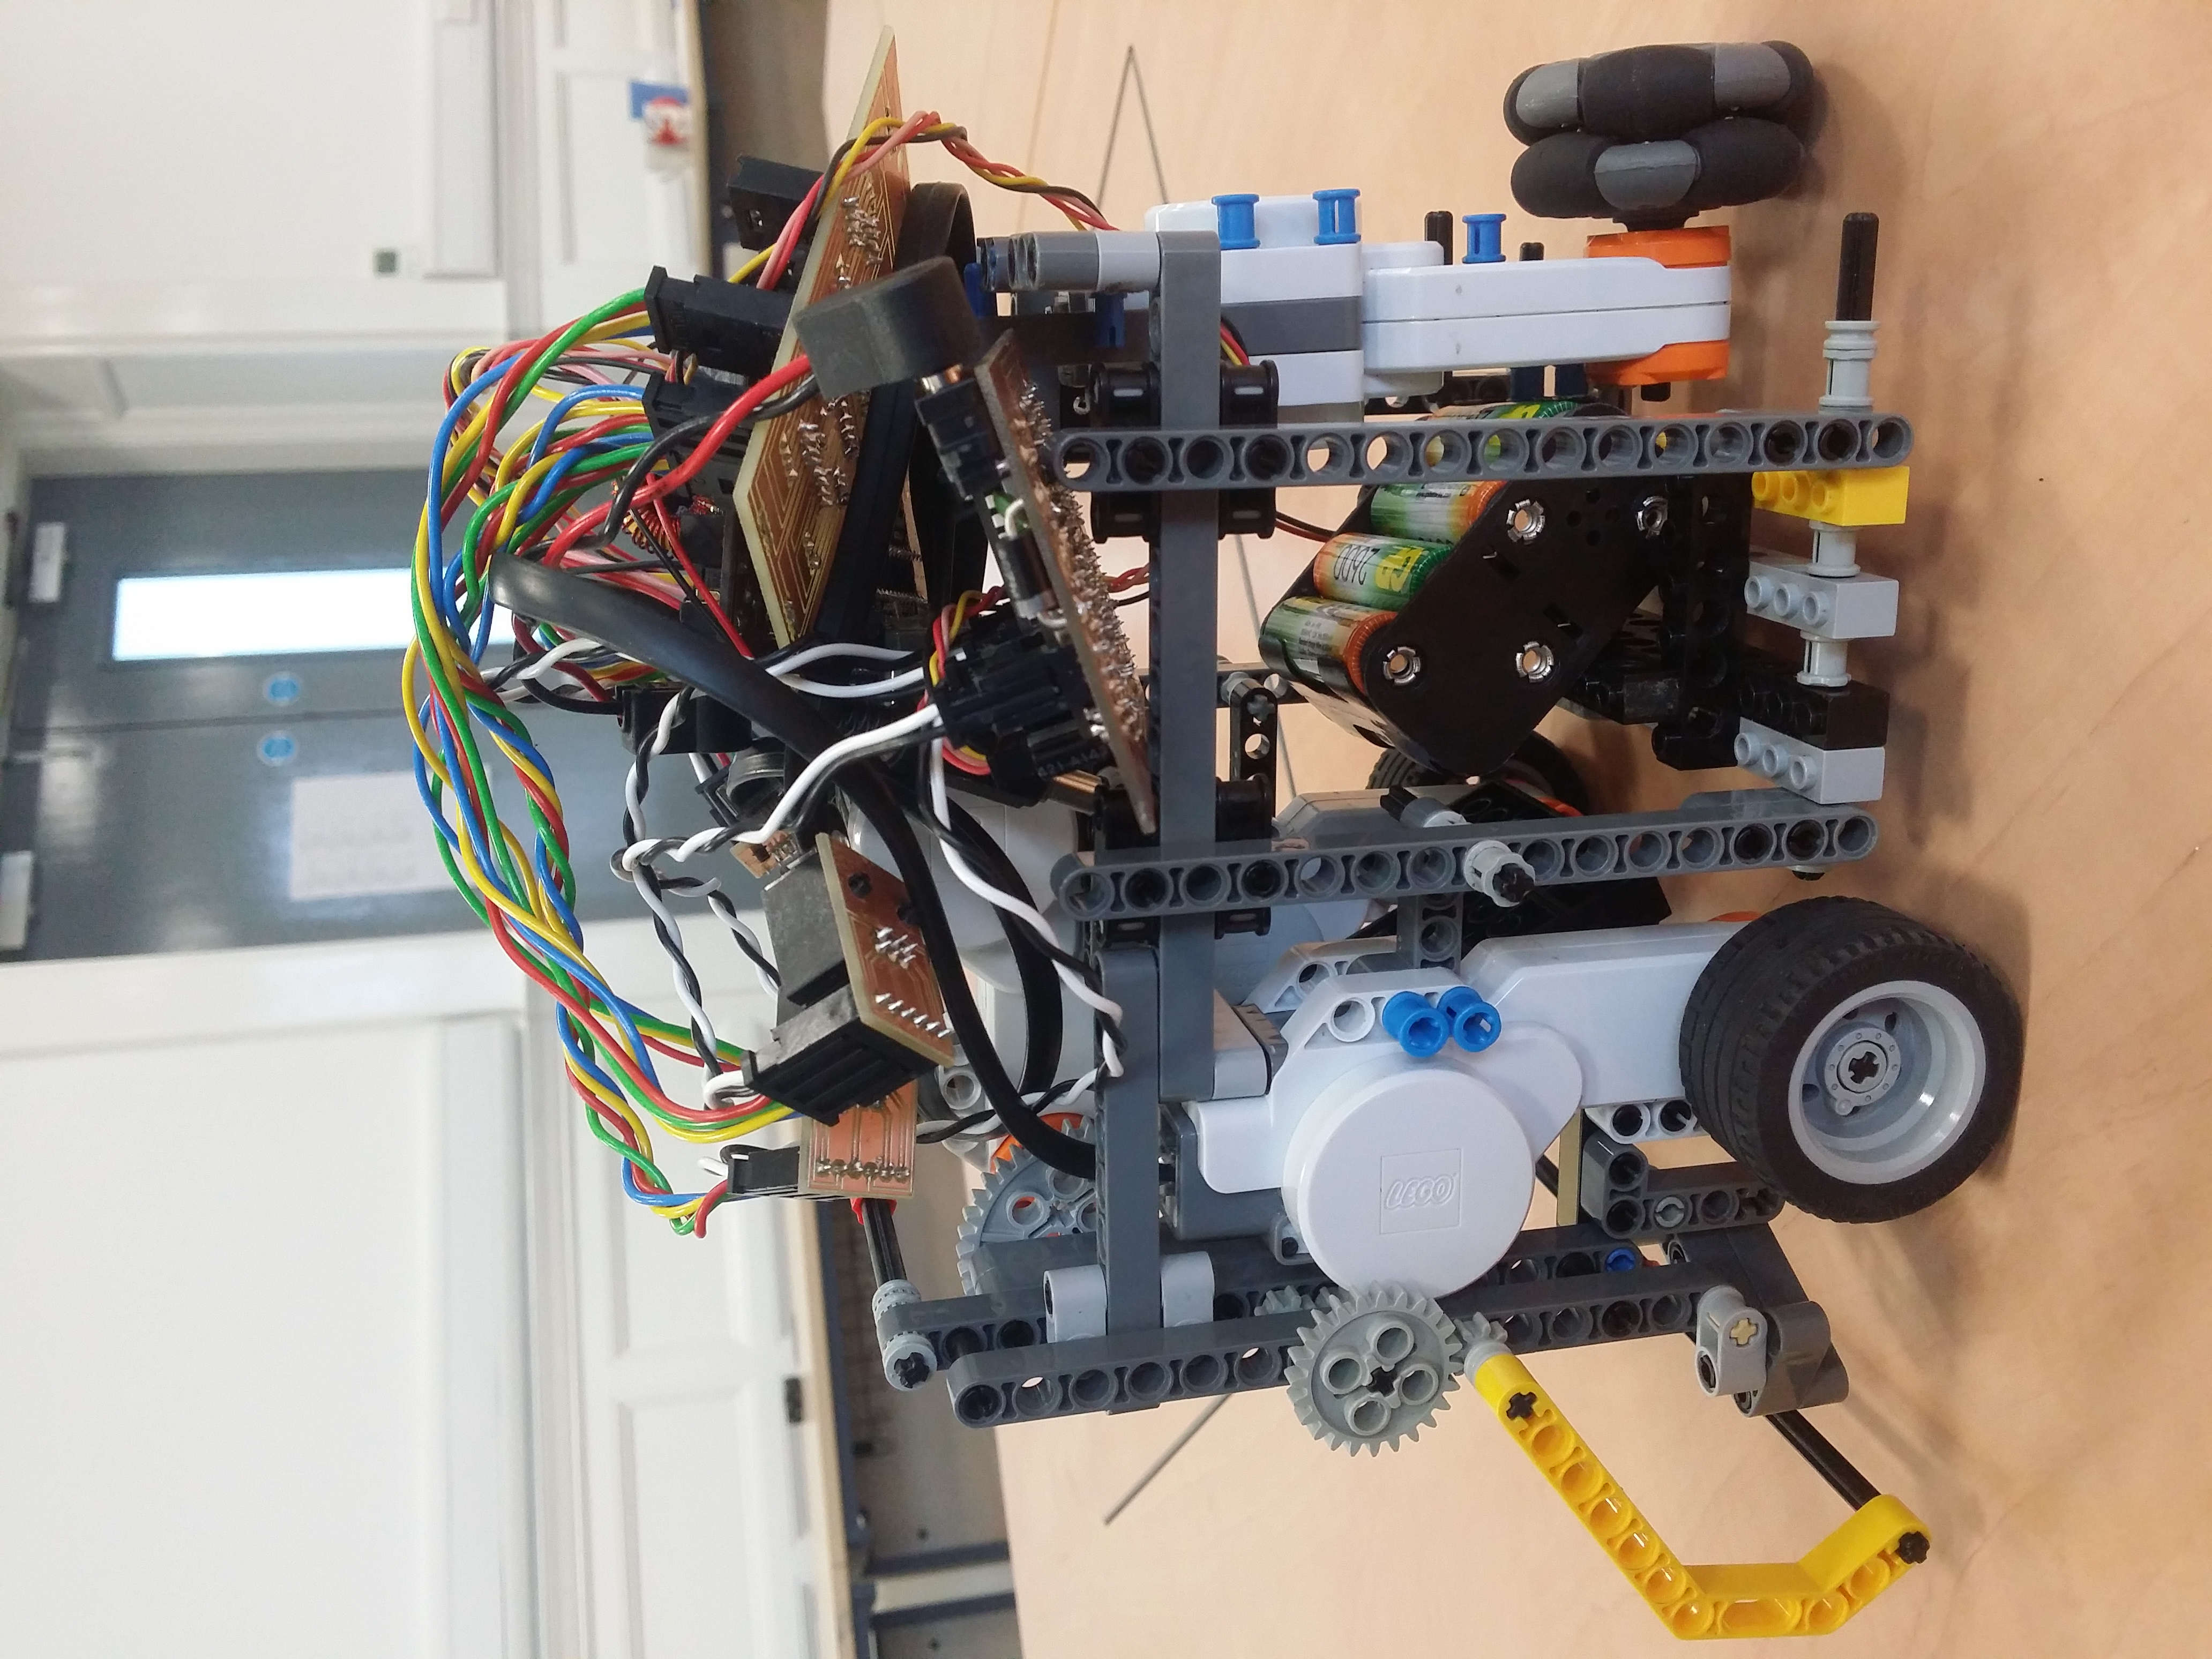
\includegraphics[scale=.07, angle = -90]{robot1.jpg} 
	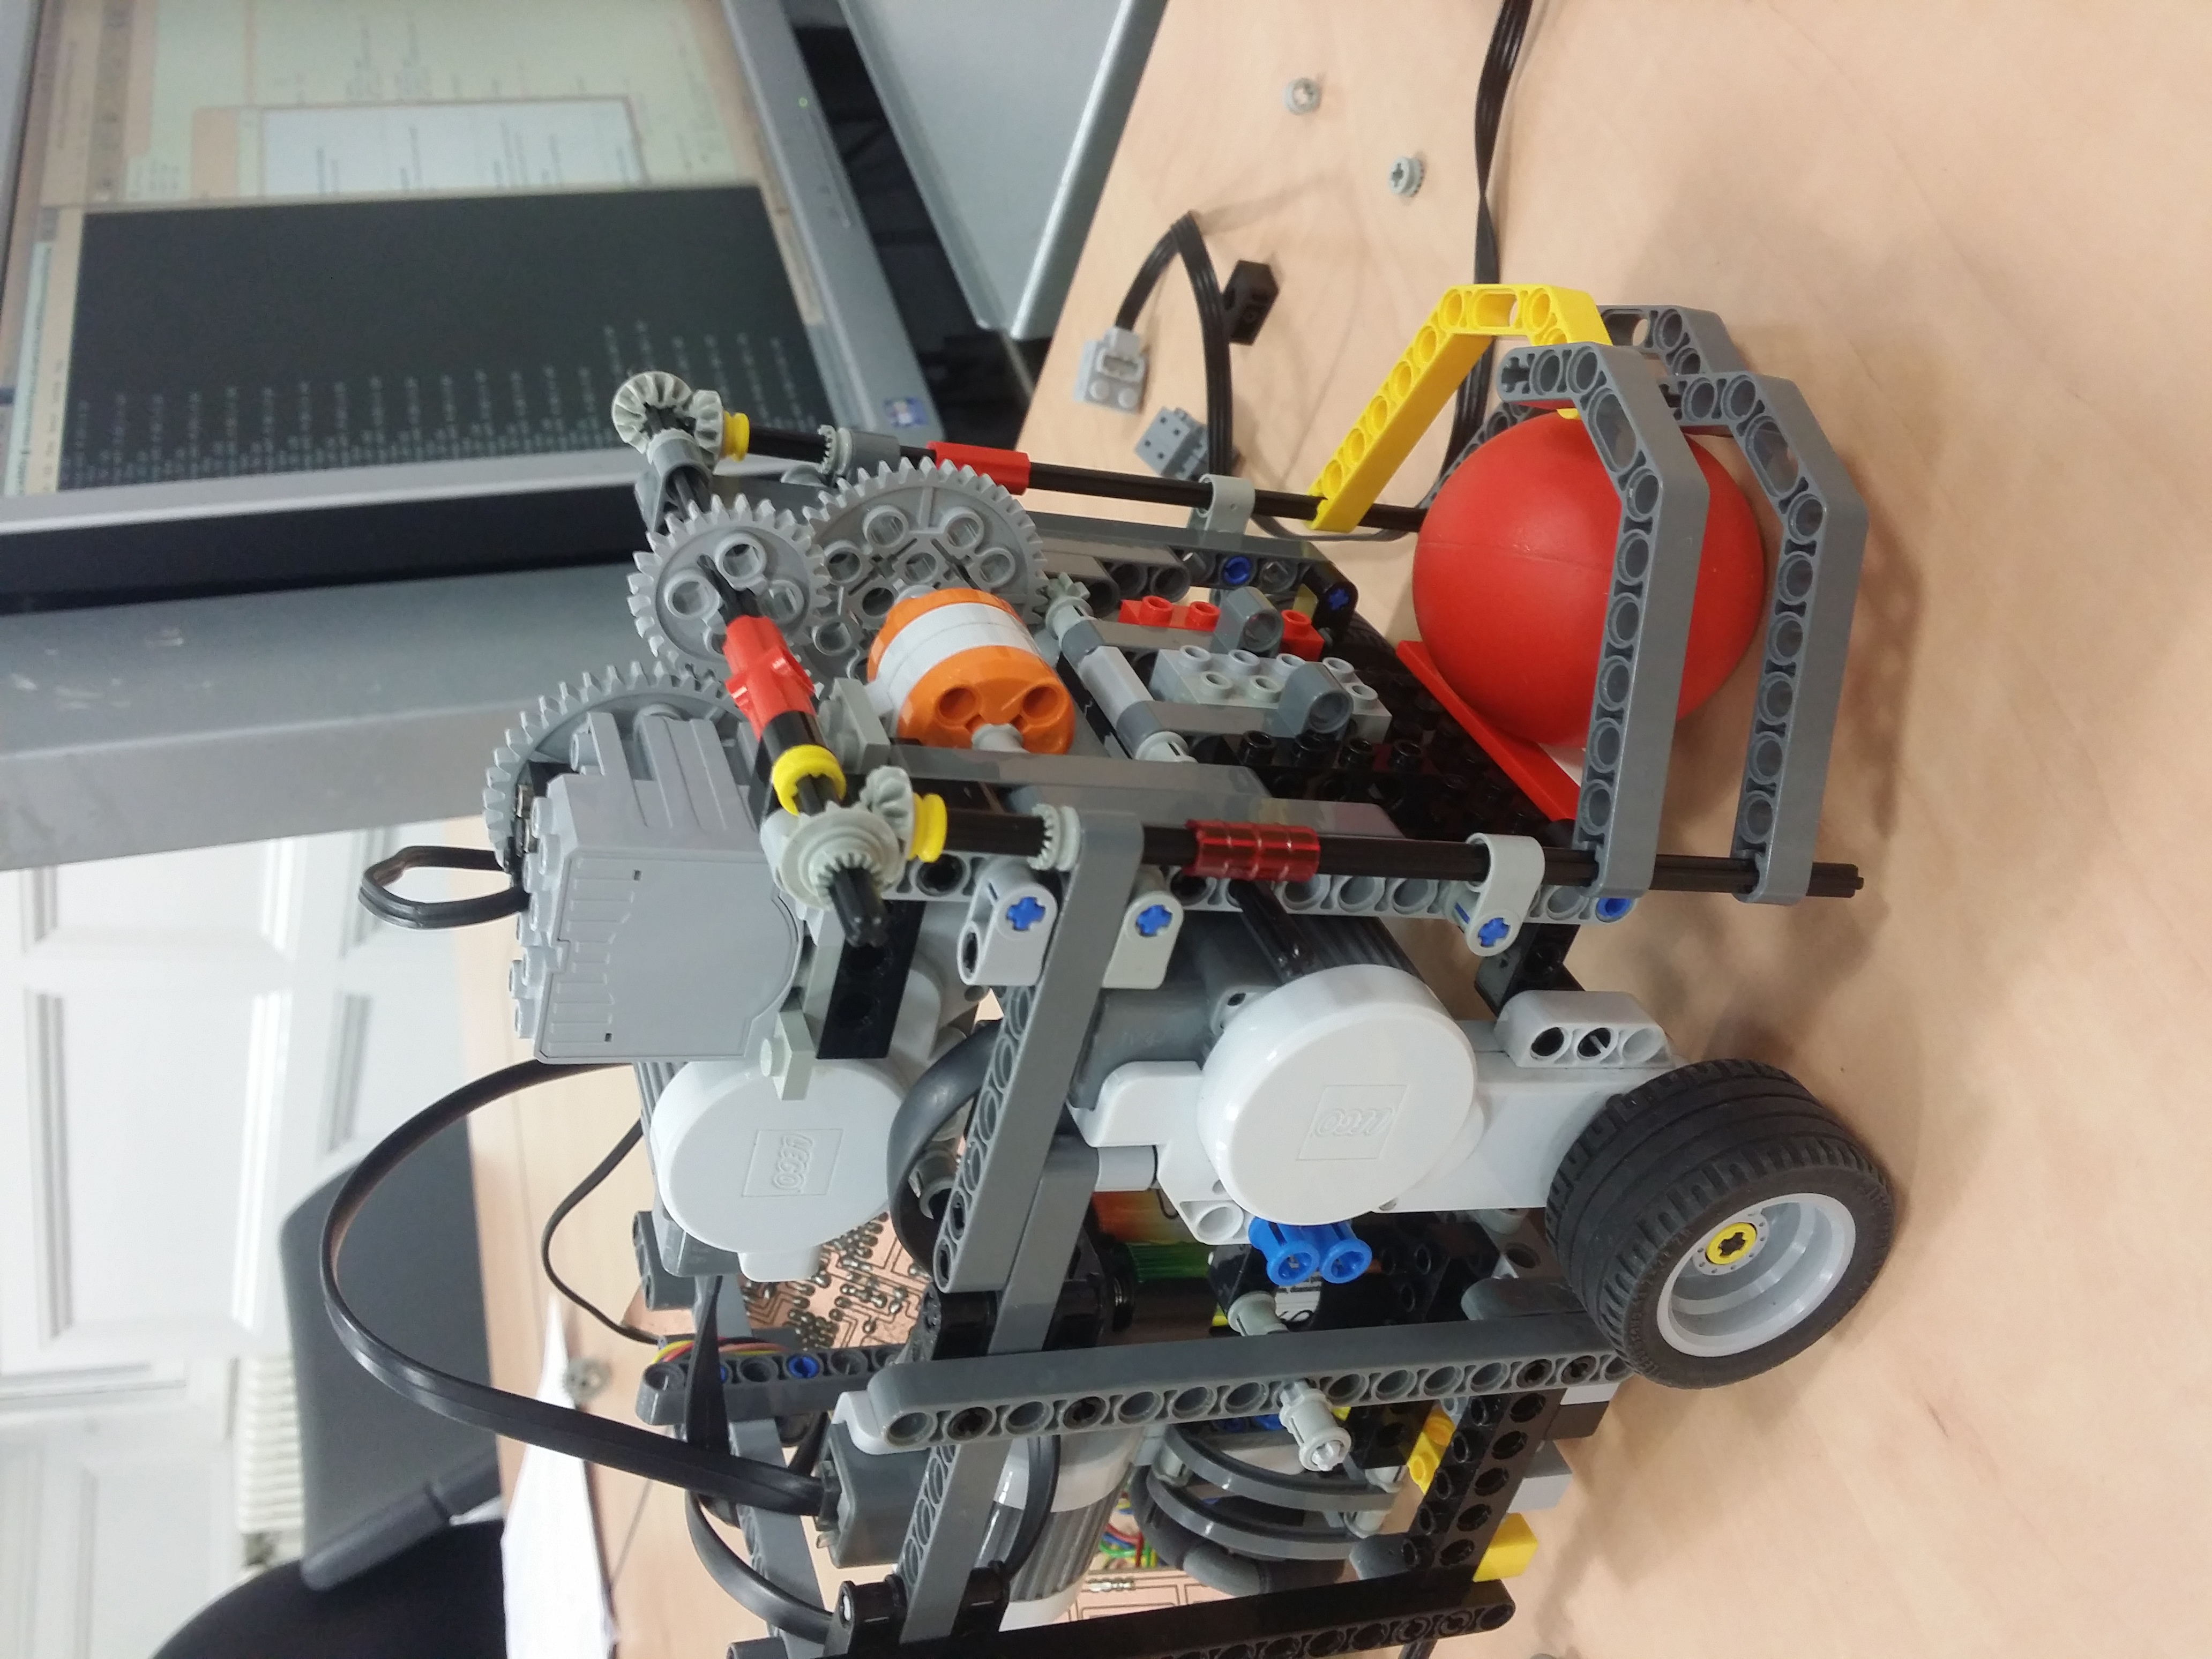
\includegraphics[scale=.07, angle = -90]{robot2.jpg}
	\bigskip

	Advantage of such design is that it is simple, but the robot can still move fast enough and we can control the power of the kick. 
 
  \section{Hardware}  
  \bigskip
  
  The initial robot had four holonomic wheels. The later design had two main wheels, and one back holonomic wheel, which allowed the robot to turn as well as move forwards/backwards without difficulties. 
	Even though we liked the idea of kicker that uses elastic (this made it more powerful). It was almost impossible to predict the distance. That's why the design that we used for the milestone has a kicker that is powered by the NXT motor and gears.
  \section{Documentation of code} 
  \bigskip
  
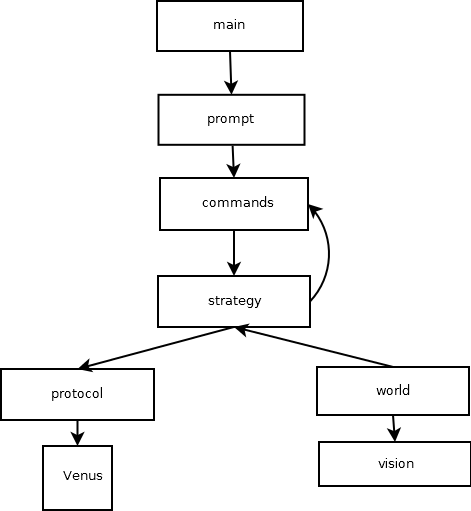
\includegraphics[scale=.7]{Diagram2}

\section{Vision, communication, planning, strategy, etc.}
	\subsection{Communication} 

		This will change soon, current commands are in User Guide.

	\subsection{Sensors} 
		\subsubsection{Rotary Encoder Board} 
			
			Each motor is connected to the rotary encoder board. This way we get to know how many rotations the motor did since the last query. After every 30ms we query the board and check if we have reached our target value or not. After the value we get becomes greater or equal to the target, we stop the motor.
 
\end{document}
